\documentclass[11pt]{article}
\usepackage[T1]{fontenc}
\usepackage[utf8]{inputenc}
\usepackage{lmodern}
\usepackage{microtype}
\usepackage{amsmath,amssymb}
\usepackage{geometry}
\usepackage{tikz}
\usetikzlibrary{arrows.meta,calc}
\geometry{letterpaper,margin=1.05in}
\setlength{\parindent}{1.15em}
\setlength{\parskip}{0pt}
\emergencystretch=2em
\allowdisplaybreaks

\newcommand{\dd}{\,d}
\newcommand{\pzero}{p^{0}}
\newcommand{\tz}{t^{0}}
\newcommand{\figlabel}[1]{\par\smallskip\centerline{\small #1}\smallskip}

\begin{document}

\begin{center}
{\large I.}\par\vspace{1.2em}
{\Large\bfseries GRAPHICAL METHODS IN THE THERMODYNAMICS\\ OF FLUIDS}\par\vspace{0.8em}
{\itshape Transactions of the Connecticut Academy}, II., pp. 309--342, April--May, 1873.
\end{center}

Although geometrical representations of propositions in the thermodynamics of fluids are in general use, and have done good service in disseminating clear notions in this science, yet they have by no means received the extension in respect to variety and generality of which they are capable. So far as regards a general graphical method, which can exhibit at once all the thermodynamic properties of a fluid concerned in reversible processes, and serve alike for the demonstration of general theorems and the numerical solution of particular problems, it is the general if not the universal practice to use diagrams in which the rectilinear co-ordinates represent volume and pressure. The object of this article is to call attention to certain diagrams of different construction, which afford graphical methods co-extensive in their applications with that in ordinary use, and preferable to it in many cases in respect of distinctness or of convenience.

\begin{center}
\bfseries Quantities and Relations which are to be represented by the Diagram.
\end{center}

We have to consider the following quantities:
\[
\left.
\begin{array}{ll}
v, & \text{the volume,}\\
p, & \text{the pressure,}\\
t, & \text{the (absolute) temperature,}\\
e, & \text{the energy,}\\
\eta, & \text{the entropy,}
\end{array}
\right\}\quad\text{of a given body in any state,}
\]
and also
\[
\left.
\begin{array}{ll}
W, & \text{the work done,}\\
H, & \text{the heat received,}
\end{array}
\right\}\quad\text{by the body in passing from one state to another.}
\]
\footnote{Work spent upon the body is as usual to be considered as a negative quantity of work done by the body, and heat given out by the body as a negative quantity of heat received by it. It is taken for granted that the body has a uniform temperature throughout, and that the pressure (or expansive force) has a uniform value both for all points in the body and for all directions. This, it will be observed, will exclude irreversible processes, but will not entirely exclude solids, although the condition of equal pressure in all directions renders the case very limited in which they come within the scope of the discussion.}

These are subject to the relations expressed by the following differential equations:
\begin{align}
dW &= \alpha p\,dv, \tag{a}\\
de &= \beta\,dH-dW, \tag{b}\\
d\eta &= \frac{dH}{t}, \tag{c}
\end{align}
where $\alpha$ and $\beta$ are constants depending upon the units by which $v,p,W$ and $H$ are measured. We may suppose our units so chosen that $\alpha=1$ and $\beta=1$, and write our equations in the simpler form,
\begin{align}
de &= dH-dW, \tag{1}\\
dW &= p\,dv, \tag{2}\\
dH &= t\,d\eta. \tag{3}
\end{align}
Eliminating $dW$ and $dH$, we have
\begin{equation}
de=t\,d\eta-p\,dv. \tag{4}
\end{equation}
The quantities $v,p,t,e$ and $\eta$ are determined when the state of the body is given, and it may be permitted to call them functions of the state of the body. The state of a body, in the sense in which the term is used in the thermodynamics of fluids, is capable of two independent variations, so that between the five quantities $v,p,t,e$ and $\eta$ there exist relations expressible by three finite equations, different in general for different substances, but always such as to be in harmony with the differential equation (4). This equation evidently signifies that if $e$ be expressed as function of $v$ and $\eta$, the partial differential co-efficients of this function taken with respect to $v$ and to $\eta$ will be equal to $-p$ and to $t$ respectively.
\footnote{Equation (a) may be derived from simple mechanical considerations. Equations (b) and (c) may be considered as defining the energy and entropy of any state of the body, or more strictly as defining the differentials $de$ and $d\eta$. That functions of the state of the body exist, the differentials of which satisfy these equations, may easily be deduced from the first and second laws of thermodynamics. The term entropy, it will be observed, is here used in accordance with the original suggestion of Clausius, and not in the sense in which it has been employed by Professor Tait and others after his suggestion. The same quantity has been called by Professor Rankine the thermodynamic function. See Clausius, \emph{Mechanische W\"armetheorie}, Abhnd. ix. \S 14; or \emph{Pogg. Ann.}, Bd. cxxv. (1865), p. 390; and Rankine, \emph{Phil. Trans.}, vol. 144, p. 126.}
\footnote{For example, we may choose as the unit of volume the cube of the unit of length, as the unit of pressure the unit of force acting upon the square of the unit of length, as the unit of work the unit of force acting through the unit of length, and as the unit of heat the thermal equivalent of the unit of work. The units of length and of force would still be arbitrary as well as the unit of temperature.}
\footnote{An equation giving $e$ in terms of $\eta$ and $v$, or more generally any finite equation between $e,\eta$ and $v$ for a definite quantity of any fluid, may be considered as the fundamental thermodynamic equation of that fluid, as from it by aid of equations (2), (3) and (4) may be derived all the thermodynamic properties of the fluid (so far as reversible processes are concerned), viz.: the fundamental equation with equation (4) gives the three relations existing between $v,p,t,e$ and $\eta$, and these relations being known, equations (2) and (3) give the work $W$ and heat $H$ for any change of state of the fluid.}

On the other hand $W$ and $H$ are not functions of the state of the body (or functions of any of the quantities $v,p,t,e$ and $\eta$), but are determined by the whole series of states through which the body is supposed to pass.

\begin{center}
\bfseries Fundamental Idea and General Properties of the Diagram.
\end{center}

Now if we associate a particular point in a plane with every separate state, of which the body is capable, in any continuous manner, so that states differing infinitely little are associated with points which are infinitely near to each other, the points associated with states of equal volume will form lines, which may be called lines of equal volume, the different lines being distinguished by the numerical value of the volume (as lines of volume 10, 20, 30, etc.). In the same way we may conceive of lines of equal pressure, of equal temperature, of equal energy, and of equal entropy. These lines we may also call isometric, isopiestic, isothermal, isodynamic, isentropic, and if necessary use these words as substantives.
\footnote{The method usually employed in treatises on thermodynamics, in which the rectangular co-ordinates of the point are made proportional to the volume and pressure of the body, is a single example of such an association.}
\footnote{These lines are usually known by the name given them by Rankine, adiabatic. If, however, we follow the suggestion of Clausius and call that quantity entropy, which Rankine called the thermodynamic function, it seems natural to go one step farther, and call the lines in which this quantity has a constant value isentropic.}

Suppose the body to change its state, the points associated with the states through which the body passes will form a line, which we may call the path of the body. The conception of a path must include the idea of direction, to express the order in which the body passes through the series of states. With every such change of state there is connected in general a certain amount of work done, $W$, and of heat received, $H$, which we may call the work and the heat of the path. The value of these quantities may be calculated from equations (2) and (3),
\begin{align*}
dW &= p\,dv, & dH &= t\,d\eta,
\end{align*}
i.e.,
\begin{align}
W &= \int p\,dv, \tag{5}\\
H &= \int t\,d\eta, \tag{6}
\end{align}
the integration being carried on from the beginning to the end of the path. If the direction of the path is reversed, $W$ and $H$ change their signs, remaining the same in absolute value.
\footnote{For the sake of brevity, it will be convenient to use language which attributes to the diagram properties which belong to the associated states of the body. Thus it can give rise to no ambiguity, if we speak of the volume or the temperature of a point in the diagram, or of the work or heat of a line, instead of the volume or temperature of the body in the state associated with the point, or the work done or the heat received by the body in passing through the states associated with the points of the line. In like manner also we may speak of the body moving along a line in the diagram, instead of passing through the series of states represented by the line.}

If the changes of state of the body form a cycle, i.e., if the final state is the same as the initial, the path becomes a circuit, and the work done and heat received are equal, as may be seen from equation (1), which when integrated for this case becomes $0=H-W$.

The circuit will enclose a certain area, which we may consider as positive or negative according to the direction of the circuit which circumscribes it. The direction in which areas must be circumscribed in order that their value may be positive, is of course arbitrary. In other words, if $x$ and $y$ are the rectangular co-ordinates, we may define an area either as $\int y\,dx$, or as $\int x\,dy$.

If an area be divided into any number of parts, the work done in the circuit bounding the whole area is equal to the sum of the work done in all the circuits bounding the partial areas. This is evident from the consideration, that the work done in each of the lines which separate the partial areas appears twice and with contrary signs in the sum of the work done in the circuits bounding the partial areas. Also the heat received in the circuit bounding the whole area is equal to the sum of the heat received in all the circuits bounding the partial areas.
\footnote{The conception of areas as positive or negative renders it unnecessary in propositions of this kind to state explicitly the direction in which the circuits are to be described. For the directions of the circuits are determined by the signs of the areas, and the signs of the partial areas must be the same as that of the area out of which they were formed.}

If all the dimensions of a circuit are infinitely small, the ratio of the included area to the work or heat of the circuit is independent of the shape of the circuit and the direction in which it is described, and varies only with its position in the diagram. That this ratio is independent of the direction in which the circuit is described, is evident from the consideration that a reversal of this direction simply changes the sign of both terms of the ratio. To prove that the ratio is independent of the shape of the circuit, let us suppose the area $ABCDE$ (fig. 1) divided up by an infinite number of isometrics $v_1v_1, v_2v_2$, etc., with equal differences of volume $dv$, and an infinite number of isopiestics $p_1p_1, p_2p_2$, etc., with equal differences of pressure $dp$. Now from the principle of continuity, as the whole figure is infinitely small, the ratio of the area of one of the small quadrilaterals into which the figure is divided to the work done in passing around it is approximately the same for all the different quadrilaterals. Therefore the area of the figure composed of all the complete quadrilaterals which fall within the given circuit has to the work done in circumscribing this figure the same ratio, which we will call $\gamma$. But the area of this figure is approximately the same as that of the given circuit, and the work done in describing this figure is approximately the same as that done in describing the given circuit (eq. 5). Therefore the area of the given circuit has to the work done or heat received in that circuit this ratio $\gamma$, which is independent of the shape of the circuit.

\begin{figure}[h]
\centering
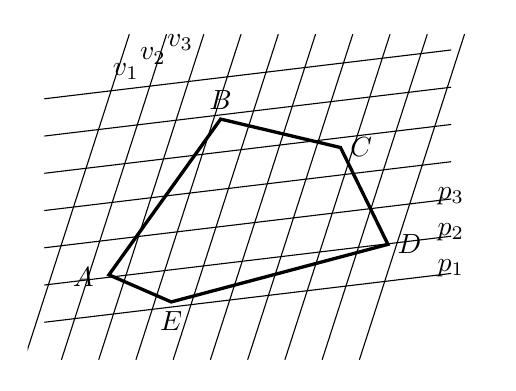
\begin{tikzpicture}[scale=.86, line cap=round]
  \clip (-.5,-1.15) rectangle (6.3,3.8);
  \foreach \i in {-1,...,8}{\draw[thin] (\i*.55,-1.1) -- ++(1.55,4.8);}
  \foreach \j in {-1,...,5}{\draw[thin] (-.25,\j*.55) -- ++(6.0,.72);}
  \draw[very thick] (.7,.15) -- (2.35,2.45) -- (4.12,2.03) -- (4.82,.6) -- (1.62,-.25) -- cycle;
  \node at (.62,.12) [left] {$A$};
  \node at (2.35,2.45) [above] {$B$};
  \node at (4.12,2.03) [right] {$C$};
  \node at (4.82,.6) [right] {$D$};
  \node at (1.62,-.25) [below] {$E$};
  \node at (.95,3.15) {$v_1$}; \node at (1.35,3.38) {$v_2$}; \node at (1.75,3.58) {$v_3$};
  \node at (5.75,.25) {$p_1$}; \node at (5.75,.78) {$p_2$}; \node at (5.75,1.31) {$p_3$};
\end{tikzpicture}
\figlabel{Fig. 1.}
\end{figure}

Now if we imagine the systems of equidifferent isometrics and isopiestics, which have just been spoken of, extended over the whole diagram, the work done in circumscribing one of the small quadrilaterals, so that the increase of pressure directly precedes the increase of volume, will have in every part of the diagram a constant value, viz., the product of the differences of volume and pressure ($dv\times dp$), as may easily be proved by applying equation (2) successively to its four sides. But the area of one of these quadrilaterals, which we could consider as constant within the limits of the infinitely small circuit, may vary for different parts of the diagram, and will indicate proportionally the value of $\gamma$, which is equal to the area divided by $dv\times dp$.

In like manner, if we imagine systems of isentropics and isothermals drawn throughout the diagram for equal differences $d\eta$ and $dt$, the heat received in passing around one of the small quadrilaterals, so that the increase of $t$ shall directly precede that of $\eta$, will be the constant product $d\eta\times dt$, as may be proved by equation (3), and the value of $\gamma$, which is equal to the area divided by the heat, will be indicated proportionally by the areas.
\footnote{The indication of the value of $\gamma$ by systems of equidifferent isometrics and isopiestics, or isentropics and isothermals, is explained above, because it seems in accordance with the spirit of the graphical method, and because it avoids the extraneous consideration of the co-ordinates. If, however, it is desired to have analytical expressions for the value of $\gamma$ based upon the relations between the co-ordinates of the point and the state of the body, it is easy to deduce such expressions as the following, in which $x$ and $y$ are the rectangular co-ordinates, and it is supposed that the sign of an area is determined in accordance with the equation $A=\int y\,dx$.}

For example, where $x$ and $y$ are regarded as the independent variables,
\begin{equation*}
\frac1\gamma=\frac{dv}{dx}\frac{dp}{dy}-\frac{dp}{dx}\frac{dv}{dy}
=\frac{dt}{dx}\frac{d\eta}{dy}-\frac{d\eta}{dx}\frac{dt}{dy};
\end{equation*}
where $v$ and $p$ are the independent variables,
\begin{equation*}
\gamma=\frac{dx}{dv}\frac{dy}{dp}-\frac{dy}{dv}\frac{dx}{dp};
\end{equation*}
where $\eta$ and $t$ are the independent variables,
\begin{equation*}
\gamma=\frac{dx}{d\eta}\frac{dy}{dt}-\frac{dy}{d\eta}\frac{dx}{dt};
\end{equation*}
and where $v$ and $\eta$ are the independent variables,
\begin{equation*}
\frac1\gamma=
\frac{-\dfrac{d^2e}{dv\,d\eta}}
{\dfrac{dx}{dv}\dfrac{dy}{d\eta}-\dfrac{dy}{dv}\dfrac{dx}{d\eta}}.
\end{equation*}

These and similar expressions for $1/\gamma$ may be found by dividing the value of the work or heat for an infinitely small circuit by the area included. This operation can be most conveniently performed upon a circuit consisting of four lines, in each of which one of the independent variables is constant. E.g., the last formula can be most easily found from an infinitely small circuit formed of two isometrics and two isentropics.

This quantity $\gamma$, which is the ratio of the area of an infinitely small circuit to the work done or heat received in that circuit, and which we may call the scale on which work and heat are represented by areas, or more briefly, the scale of work and heat, may have a constant value throughout the diagram or it may have a varying value. The diagram in ordinary use affords an example of the first case, as the area of a circuit is everywhere proportional to the work or heat. There are other diagrams which have the same property, and we may call all such diagrams of constant scale.

In any case we may consider the scale of work and heat as known for every point of the diagram, so far as we are able to draw the isometrics and isopiestics or the isentropics and isothermals. If we write $\delta W$ and $\delta H$ for the work and heat of an infinitesimal circuit, and $\delta A$ for the area included, the relations of these quantities are thus expressed:
\begin{equation}
\delta W=\delta H=\frac1\gamma\,\delta A. \tag{7}
\end{equation}
\footnote{To avoid confusion, as $dW$ and $dH$ are generally used and are used elsewhere in this article to denote the work and heat of an infinitely short path, a slightly different notation, $\delta W$ and $\delta H$, is here used to denote the work and heat of an infinitely small circuit. So $\delta A$ is used to denote an element of area which is infinitely small in all directions, as the letter $d$ would only imply that the element was infinitely small in one direction. So also below, the integration or summation which extends to all the elements written with $\delta$ is denoted by the character $\Sigma$, as the character $\int$ naturally refers to elements written with $d$.}

We may find the value of $W$ and $H$ for a circuit of finite dimensions by supposing the included area $A$ divided into areas $\delta A$ infinitely small in all directions, for which therefore the above equation will hold, and taking the sum of the values of $\delta H$ or $\delta W$ for the various areas $\delta A$. Writing $W^C$ and $H^C$ for the work and heat of the circuit $C$, and $\Sigma^C$ for a summation or integration performed within the limits of this circuit, we have
\begin{equation}
W^C=H^C=\Sigma^C \frac1\gamma\,\delta A. \tag{8}
\end{equation}
We have thus an expression for the value of the work and heat of a circuit involving an integration extending over an area instead of one extending over a line, as in equations (5) and (6).

Similar expressions may be found for the work and the heat of a path which is not a circuit. For this case may be reduced to the preceding by the consideration that $W=0$ for a path on an isometric or on the line of no pressure (eq. 2), and $H=0$ for a path on an isentropic or on the line of absolute cold. Hence the work of any path $S$ is equal to that of the circuit formed of $S$, the isometric of the final state, the line of no pressure and the isometric of the initial state, which circuit may be represented by the notation $[S,v'',p^0,v']$. And the heat of the same path is the same as that of the circuit $[S,\eta'',t^0,\eta']$. Therefore using $W^S$ and $H^S$ to denote the work and heat of any path $S$, we have
\begin{align}
W^S&=\Sigma^{[S,v'',p^0,v']}\frac1\gamma\,\delta A, \tag{9}\\
H^S&=\Sigma^{[S,\eta'',t^0,\eta']}\frac1\gamma\,\delta A, \tag{10}
\end{align}
where as before the limits of the integration are denoted by the expression occupying the place of an index to the sign $\Sigma$.
\footnote{A word should be said in regard to the sense in which the above propositions should be understood. If beyond the limits, within which the relations of $v,p,t,e$ and $\eta$ are known and which we may call the limits of the known field, we continue the isometrics, isopiestics, etc., in any way we please, only subject to the condition that the relations of $v,p,t,e$ and $\eta$ shall be consistent with the equation $de=t\,d\eta-p\,dv$, then in calculating the values of quantities $W$ and $H$ determined by the equations $dW=p\,dv$ and $dH=t\,d\eta$ for paths or circuits in any part of the diagram thus extended, we may use any of the propositions or processes given above, as these three equations have formed the only basis of the reasoning. We will thus obtain values of $W$ and $H$, which will be identical with those which would be obtained by the immediate application of the equations $dW=p\,dv$ and $dH=t\,d\eta$ to the path in question, and which in the case of any path which is entirely contained in the known field will be the true values of the work and heat for the change of state of the body which the path represents. We may thus use lines outside of the known field without attributing to them any physical signification whatever, without considering the points in the lines as representing any states of the body. If however, to fix our ideas, we choose to conceive of this part of the diagram as having the same physical interpretation as the known field, and to enunciate our propositions in language based upon such a conception, the unreality or even the impossibility of the states represented by the lines outside of the known field cannot lead to any incorrect results in regard to paths in the known field.}

It is easy to form a material conception of these relations. If we imagine, for example, mass inherent in the plane of the diagram with a varying (superficial) density represented by $1/\gamma$, then $\Sigma (1/\gamma)\delta A$ will evidently denote the mass of the part of the plane included within the limits of integration, this mass being taken positively or negatively according to the direction of the circuit.

Thus far we have made no supposition in regard to the nature of the law, by which we associate the points of a plane with the states of the body, except a certain condition of continuity. Whatever law we may adopt, we obtain a method of representation of the thermodynamic properties of the body, in which the relations existing between the functions of the state of the body are indicated by a net-work of lines, while the work done and the heat received by the body when it changes its state are represented by integrals extending over the elements of a line, and also by an integral extending over the elements of certain areas in the diagram, or, if we choose to introduce such a consideration, by the mass belonging to these areas.

The different diagrams which we obtain by different laws of association are all such as may be obtained from one another by a process of deformation, and this consideration is sufficient to demonstrate their properties from the well-known properties of the diagram in which the volume and pressure are represented by rectangular co-ordinates. For the relations indicated by the net-work of isometrics, isopiestics etc., are evidently not altered by deformation of the surface upon which they are drawn, and if we conceive of mass as belonging to the surface, the mass included within given lines will also not be affected by the process of deformation. If, then, the surface upon which the ordinary diagram is drawn has the uniform superficial density 1, so that the work and heat of a circuit, which are represented in this diagram by the included area, shall also be represented by the mass included, this latter relation will hold for any diagram formed from this by deformation of the surface on which it is drawn.

The choice of the method of representation is of course to be determined by considerations of simplicity and convenience, especially in regard to the drawing of the lines of equal volume, pressure, temperature, energy and entropy, and the estimation of work and heat. There is an obvious advantage in the use of diagrams of constant scale, in which the work and heat are represented simply by areas. Such diagrams may of course be produced by an infinity of different methods, as there is no limit to the ways of deforming a plane figure without altering the magnitude of its elements. Among these methods, two are especially important,---the ordinary method in which the volume and pressure are represented by rectilinear co-ordinates, and that in which the entropy and temperature are so represented. A diagram formed by the former method may be called, for the sake of distinction, a volume-pressure diagram,---one formed by the latter, an entropy-temperature diagram. That the latter as well as the former satisfies the condition that $\gamma=1$ throughout the whole diagram, may be seen by reference to page 5.

\begin{center}
\bfseries The Entropy-temperature Diagram compared with that in ordinary use.
\end{center}
\begin{center}
\itshape Considerations independent of the nature of the body in question.
\end{center}

As the general equations (1), (2), (3) are not altered by interchanging $v,-p$ and $-W$ with $\eta,t$ and $H$ respectively, it is evident that, so far as these equations are concerned, there is nothing to choose between a volume-pressure and an entropy-temperature diagram. In the former, the work is represented by an area bounded by the path which represents the change of state of the body, two ordinates and the axis of abscissas. The same is true of the heat received in the latter diagram. Again, in the former diagram, the heat received is represented by an area bounded by the path and certain lines, the character of which depends upon the nature of the body under consideration. Except in the case of an ideal body, the properties of which are determined by assumption, these lines are more or less unknown in a part of their course, and in any case the area will generally extend to an infinite distance. Very much the same inconveniences attach themselves to the areas representing work in the entropy-temperature diagram.
\footnote{In neither diagram do these circumstances create any serious difficulty in the estimation of areas representing work or heat. It is always possible to divide these areas into two parts, of which one is of finite dimensions, and the other can be calculated in the simplest manner. Thus in the entropy-temperature diagram the work done in a path $AB$ (fig. 2) is represented by the area included by the path $AB$, the isometric $BC$, the line of no pressure and the isometric $DA$. The line of no pressure and the adjacent parts of the isometrics in the case of an actual gas or vapor are more or less undetermined in the present state of our knowledge, and are likely to remain so; for an ideal gas the line of no pressure coincides with the axis of abscissas, and is an asymptote to the isometrics. But, be this as it may, it is not necessary to examine the form of the remoter parts of the diagram. If we draw an isopiestic $MN$, cutting $AD$ and $BC$, the area $MNCD$, which represents the work done in $MN$, will be equal to $p(v''-v')$, where $p$ denotes the pressure in $MN$, and $v''$ and $v'$ denote the volumes at $B$ and $A$ respectively (eq. 5). Hence the work done in $AB$ will be represented by $ABNM+p(v''-v')$. In the volume-pressure diagram, the areas representing heat may be divided by an isothermal, and treated in a manner entirely analogous. Or we may make use of the principle that, for a path which begins and ends on the same isodynamic, the work and heat are equal, as appears by integration of equation (1). Hence, in the entropy-temperature diagram, to find the work of any path, we may extend it by an isometric (which will not alter its work), so that it shall begin and end on the same isodynamic, and then take the heat (instead of the work) of the path thus extended. This method was suggested by that employed by Cazin, \emph{Th\'eorie \'el\'ementaire des machines \`a air chaud}, p. 11, and Zeuner, \emph{Mechanische W\"armetheorie}, p. 80, in the reverse case, viz.: to find the heat of a path in the volume-pressure diagram.}

\begin{figure}[h]
\centering
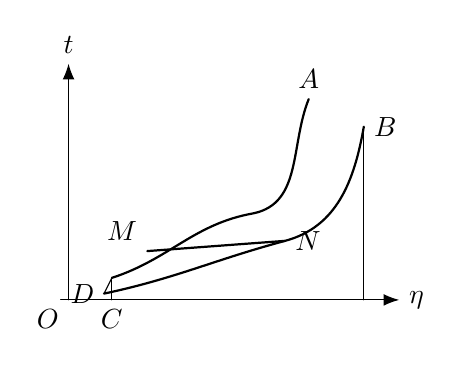
\begin{tikzpicture}[scale=1.0, line cap=round]
\draw[-{Latex[length=2mm]}] (0,0) -- (0,3.0) node[above] {$t$};
\draw[-{Latex[length=2mm]}] (-.1,0) -- (4.2,0) node[right] {$\eta$};
\node[below left] at (0,0) {$O$};
\draw[thick] (.55,.28) to[out=18,in=190] (2.35,1.1) to[out=12,in=-112] (3.05,2.55) node[above] {$A$};
\draw[thick] (.45,.08) to[out=12,in=195] (2.75,.75) node[right] {$N$} to[out=15,in=-100] (3.75,2.2) node[right] {$B$};
\draw[thin] (.55,.28) -- (.55,0) node[below] {$C$};
\draw[thin] (3.75,2.2) -- (3.75,0);
\draw[thin] (.55,.28) -- (.45,.08) node[left] {$D$};
\draw[thick] (1.0,.62) node[above left] {$M$} -- (2.75,.75);
\figlabel{Fig. 2.}
\end{tikzpicture}
\end{figure}

There is, however, a consideration of a general character, which shows an important advantage on the side of the entropy-temperature diagram. In thermodynamic problems, heat received at one temperature is by no means the equivalent of the same amount of heat received at another temperature. For example, a supply of a million calories at $150^{\circ}\mathrm{C}$ is a very different thing from a supply of a million calories at $50^{\circ}\mathrm{C}$. But no such distinction exists in regard to work. This is a result of the general law, that heat can only pass from a hotter to a colder body, while work can be transferred by mechanical means from one fluid to any other, whatever may be the pressures. Hence, in thermodynamic problems, it is generally necessary to distinguish between the quantities of heat received or given out by the body at different temperatures, while as far as work is concerned, it is generally sufficient to ascertain the total amount performed. If, then, several heat-areas and one work-area enter into the problem, it is evidently more important that the former should be simple in form, than that the latter should be so. Moreover, in the very common case of a circuit, the work-area is bounded entirely by the path, and the form of the isometrics and the line of no pressure are of no especial consequence.

It is worthy of notice that the simplest form of a perfect thermodynamic engine, so often described in treatises on thermodynamics, is represented in the entropy-temperature diagram by a figure of extreme simplicity, viz.: a rectangle of which the sides are parallel to the co-ordinate axes. Thus in figure 3, the circuit $ABCD$ may represent the series of states through which the fluid is made to pass in such an engine, the included area representing the work done, while the area $ABFE$ represents the heat received from the heater at the highest temperature $AE$, and the area $CDEF$ represents the heat transmitted to the cooler at the lowest temperature $DE$.

\begin{figure}[h]
\centering
\begin{tikzpicture}[scale=1.0, line cap=round]
\draw[-{Latex[length=2mm]}] (0,0) -- (0,3.0) node[above] {$t$};
\draw[-{Latex[length=2mm]}] (-.1,0) -- (4.3,0) node[right] {$\eta$};
\node[below left] at (0,0) {$O$};
\draw[thick] (1.75,.2) rectangle (3.0,2.35);
\draw[thin] (1.75,1.25) -- (3.0,1.25);
\node[above] at (1.75,2.35) {$A$};
\node[above] at (3.0,2.35) {$B$};
\node[right] at (3.0,1.25) {$C$};
\node[left] at (1.75,1.25) {$D$};
\node[below] at (1.75,.2) {$E$};
\node[below] at (3.0,.2) {$F$};
\figlabel{Fig. 3.}
\end{tikzpicture}
\end{figure}

There is another form of the perfect thermodynamic engine, viz.: one with a perfect regenerator as defined by Rankine, \emph{Phil. Trans.} vol. 144, p. 140, the representation of which becomes peculiarly simple in the entropy-temperature diagram. The circuit consists of two equal straight lines $AB$ and $CD$ (fig. 4) parallel to the axis of abscissas, and two precisely similar curves of any form $BC$ and $AD$.


The included area $ABCD$ represents the work done, and the areas $ABba$ and $CDdc$ represent respectively the heat received from the heater and that transmitted to the cooler. The heat imparted by the fluid to the regenerator in passing from $B$ to $C$, and afterward restored to the fluid in its passage from $D$ to $A$, is represented by the areas $BCcb$ and $DAad$.


\begin{center}
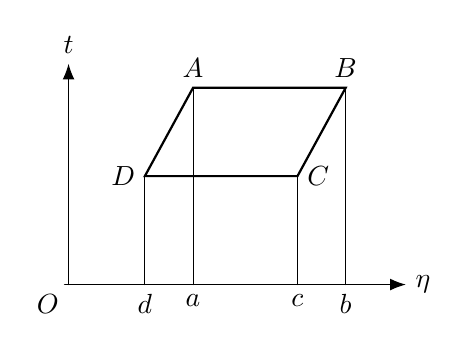
\begin{tikzpicture}[scale=1.02, line cap=round]
\draw[-{Latex[length=2mm]}] (0,0) -- (0,2.75) node[above] {$t$};
\draw[-{Latex[length=2mm]}] (-.05,0) -- (4.2,0) node[right] {$\eta$};
\node[below left] at (0,0) {$O$};
\coordinate (d) at (.95,0);
\coordinate (a) at (1.55,0);
\coordinate (c) at (2.85,0);
\coordinate (b) at (3.45,0);
\coordinate (D) at (.95,1.35);
\coordinate (A) at (1.55,2.45);
\coordinate (C) at (2.85,1.35);
\coordinate (B) at (3.45,2.45);
\draw[thin] (d) -- (D);
\draw[thin] (a) -- (A);
\draw[thin] (c) -- (C);
\draw[thin] (b) -- (B);
\draw[thick] (D) -- (A) -- (B) -- (C) -- cycle;
\node[left] at (D) {$D$};
\node[above] at (A) {$A$};
\node[above] at (B) {$B$};
\node[right] at (C) {$C$};
\node[below] at (d) {$d$};
\node[below] at (a) {$a$};
\node[below] at (c) {$c$};
\node[below] at (b) {$b$};
\figlabel{Fig. 4.}
\end{tikzpicture}
\end{center}


It is often a matter of the first importance in the study of any thermodynamic engine, to compare it with a perfect engine. Such a comparison will obviously be much facilitated by the use of a method in which the perfect engine is represented by such simple forms.

The method in which the co-ordinates represent volume and pressure has a certain advantage in the simple and elementary character of the notions upon which it is based, and its analogy with Watt's indicator has doubtless contributed to render it popular. On the other hand, a method involving the notion of \emph{entropy}, the very existence of which depends upon the second law of thermodynamics, will doubtless seem to many far-fetched, and may repel beginners as obscure and difficult of comprehension. This inconvenience is perhaps more than counterbalanced by the advantages of a method which makes the second law of thermodynamics so prominent, and gives it so clear and elementary an expression. The fact, that the different states of a fluid can be represented by the positions of a point in a plane, so that the ordinates shall represent the temperatures, and the heat received or given out by the fluid shall be represented by the area bounded by the line representing the states through which the body passes, the ordinates drawn through the extreme points of this line, and the axis of abscissas,--this fact, clumsy as its expression in words may be, is one which presents a clear image to the eye, and which the mind can readily grasp and retain. It is, however, nothing more nor less than a geometrical expression of the second law of thermodynamics in its application to fluids, in a form exceedingly convenient for use, and from which the analytical expression of the same law can, if desired, be at once obtained. If, then, it is more important for purposes of instruction and the like to familiarize the learner with the second law, than to defer its statement as long as possible, the use of the entropy-temperature diagram may serve a useful purpose in the popularizing of this science.

The foregoing considerations are in the main of a general character, and independent of the nature of the substance to which the graphical method is applied. On this, however, depend the forms of the isometrics, isopiestics and isodynamics in the entropy-temperature diagram, and of the isentropics, isothermals and isodynamics in the volume-pressure diagram. As the convenience of a method depends largely upon the ease with which these lines can be drawn, and upon the peculiarities of the fluid which has its properties represented in the diagram, it is desirable to compare the methods under consideration in some of their most important applications. We will commence with the case of a perfect gas.

\begin{center}
\itshape Case of a perfect gas.
\end{center}

A perfect or ideal gas may be defined as such a gas, that for any constant quantity of it the product of the volume and the pressure varies as the temperature, and the energy varies as the temperature, i.e.,
\begin{align}
pv&=at, \tag{A}\\
e&=ct. \tag{B}
\end{align}
\footnote{In this article, all equations which are designated by arabic numerals subsist for any body whatever (subject to the condition of uniform pressure and temperature), and those which are designated by small capitals subsist for any quantity of a perfect gas as defined above (subject of course to the same conditions).}
The significance of the constant $a$ is sufficiently indicated by equation (A). The significance of $c$ may be rendered more evident by differentiating equation (B) and comparing the result
\[
de=c\,dt
\]
with the general equations (1) and (2), viz.:
\[
de=dH-dW,\qquad dW=p\,dv.
\]
If $dv=0$, $dW=0$, and $dH=c\,dt$, i.e.,
\begin{equation}
\left(\frac{dH}{dt}\right)_v=c,\tag{C}
\end{equation}
\footnote{A subscript letter after a differential co-efficient is used in this article to indicate the quantity which is made constant in the differentiation.}
i.e., $c$ is the quantity of heat necessary to raise the temperature of the body one degree under the condition of constant volume. It will be observed, that when different quantities of the same gas are considered, $a$ and $c$ both vary as the quantity, and $c\div a$ is constant; also, that the value of $c\div a$ for different gases varies as their specific heat determined for equal volumes and for constant volume.

With the aid of equations (A) and (B) we may eliminate $p$ and $t$ from the general equation (4), viz.:
\[
de=t\,d\eta-p\,dv,
\]
which is then reduced to
\[
\frac{de}{e}=\frac{1}{c}\,d\eta-\frac{a}{c}\frac{dv}{v},
\]
and by integration to
\begin{equation}
\log e=\frac{\eta}{c}-\frac{a}{c}\log v.\tag{D}
\end{equation}
\footnote{If we use the letter $\epsilon$ to denote the base of the Naperian system of logarithms, equation (D) may also be written in the form
\[
e=\epsilon^{\eta/c}v^{-a/c}.
\]
This may be regarded as the fundamental thermodynamic equation of an ideal gas. See the last note on page 2. It will be observed, that there would be no real loss of generality if we should choose, as the body to which the letters refer, such a quantity of the gas that one of the constants $a$ and $c$ should be equal to unity.}
The constant of integration becomes $0$, if we call the entropy $0$ for the state of which the volume and energy are both unity.

Any other equations which subsist between $v,p,t,e$ and $\eta$ may be derived from the three independent equations (A), (B) and (D). If we eliminate $e$ from (B) and (D), we have
\begin{equation}
\eta=a\log v+c\log t+c\log c. \tag{E}
\end{equation}
Eliminating $v$ from (A) and (E), we have
\begin{equation}
\eta=(a+c)\log t-a\log p+c\log c+a\log a. \tag{F}
\end{equation}
Eliminating $t$ from (A) and (E), we have
\begin{equation}
\eta=(a+c)\log v+c\log p+c\log\frac{c}{a}. \tag{G}
\end{equation}

If $v$ is constant, equation (E) becomes
\[
\eta=c\log t+\mathrm{Const.},
\]
i.e., the isometrics in the entropy-temperature diagram are logarithmic curves identical with one another in form,--a change in the value of $v$ having only the effect of moving the curve parallel to the axis of $\eta$. If $p$ is constant, equation (F) becomes
\[
\eta=(a+c)\log t+\mathrm{Const.},
\]
so that the isopiestics in this diagram have similar properties. This identity in form diminishes greatly the labour of drawing any considerable number of these curves. For if a card or thin board be cut in the form of one of them, it may be used as a pattern or ruler to draw all of the same system. The isodynamics are straight in this diagram (eq. B).

To find the form of the isothermals and isentropics in the volume-pressure diagram, we may make $t$ and $\eta$ constant in equations (A) and (G) respectively, which will then reduce to the well-known equations of these curves:
\[
pv=\mathrm{Const.},
\]
and
\[
p^c v^{a+c}=\mathrm{Const.}
\]
The equation of the isodynamics is of course the same as that of the isothermals. None of these systems of lines have that property of identity of form, which makes the systems of isometrics and isopiestics so easy to draw in the entropy-temperature diagram.

\begin{center}
\itshape Case of condensable vapors.
\end{center}

The case of bodies which pass from the liquid to the gaseous condition is next to be considered. It is usual to assume of such a body, that when sufficiently superheated it approaches the condition of a perfect gas. If, then, in the entropy-temperature diagram of such a body we draw systems of isometrics, isopiestics and isodynamics, as if for a perfect gas, for proper values of the constants $a$ and $c$, these will be asymptotes to the true isometrics, etc., of the vapor, and in many cases will not vary from them greatly in the part of the diagram which represents vapor unmixed with liquid, except in the vicinity of the line of saturation. In the volume-pressure diagram of the same body, the isothermals, isentropics and isodynamics, drawn for a perfect gas for the same values of $a$ and $c$, will have the same relations to the true isothermals, etc.

In that part of any diagram which represents a mixture of vapor and liquid, the isopiestics and isothermals will be identical, as the pressure is determined by the temperature alone. In both the diagrams which we are now comparing, they will be straight and parallel to the axis of abscissas. The form of the isometrics and isodynamics in the entropy-temperature diagram, or that of the isentropics and isodynamics in the volume-pressure diagram, will depend upon the nature of the fluid, and probably cannot be expressed by any simple equations. The following property, however, renders it easy to construct equidifferent systems of these lines, viz.: any such system will divide any isothermal (isopiestic) into equal segments.

It remains to consider that part of the diagram which represents the body when entirely in the condition of liquid. The fundamental characteristic of this condition of matter is that the volume is very nearly constant, so that variations of volume are generally entirely inappreciable when represented graphically on the same scale on which the volume of the body in the state of vapor is represented, and both the variations of volume and the connected variations of the connected quantities may be, and generally are, neglected by the side of the variations of the same quantities which occur when the body passes to the state of vapor. Let us make, then, the usual assumption that $v$ is constant, and see how the general equations (1), (2), (3) and (4) are thereby affected.

We have first,
\[
dv=0,
\]
then
\[
dW=0,
\]
and
\[
de=t\,d\eta.
\]
If we add
\[
dH=t\,d\eta,
\]
these four equations will evidently be equivalent to the three independent equations (1), (2) and (3), combined with the assumption which we have just made. For a liquid, then, $e$, instead of being a function of two quantities $v$ and $\eta$, is a function of $\eta$ alone,--$t$ is also a function of $\eta$ alone, being equal to the differential co-efficient of the function $e$; that is, the value of one of the three quantities $t,e$ and $\eta$, is sufficient to determine the other two. The value of $v$, moreover, is fixed without reference to the values of $t,e$ and $\eta$ (so long as these do not pass the limits of values possible for liquidity); while $p$ does not enter into the equations, i.e., $p$ may have any value (within certain limits) without affecting the values of $t,e,\eta$ or $v$. If the body change its state, continuing always liquid, the value of $W$ for such a change is 0, and that of $H$ is determined by the values of any one of the three quantities $t,e$ and $\eta$. It is, therefore, the relations between $t,e,\eta$ and $H$, for which a graphical expression is to be sought; a method, therefore, in which the co-ordinates of the diagram are made equal to the volume and pressure, is totally inapplicable to this particular case; $v$ and $p$ are indeed the only two of the five functions of the state of the body, $v,p,t,e$ and $\eta$, which have no relations either to each other, or to the other three, or to the quantities $W$ and $H$, to be expressed.\footnote{That is, $v$ and $p$ have no such relations to the other quantities, as are expressible by equations; $p$, however, cannot be less than a certain function of $t$.} The values of $v$ and $p$ do not really determine the state of an incompressible fluid,--the values of $t,e$ and $\eta$ are still left undetermined, so that through every point in the volume-pressure diagram which represents the liquid there must pass (in general) an infinite number of isothermals, isodynamics and isentropics. The character of this part of the diagram is as follows:--the states of liquidity are represented by the points of a line parallel to the axis of pressures, and the isothermals, isodynamics and isentropics, which cross the field of partial vaporization and meet this line, turn upward and follow its course.\footnote{All these difficulties are of course removed when the differences of volume of the liquid at different temperatures are rendered appreciable on the volume-pressure diagram. This can be done in various ways,--among others, by choosing as the body to which $v$, etc., refer, a sufficiently large quantity of the fluid. But, however we do it, we must evidently give up the possibility of representing the body in the state of vapor in the same diagram without making its dimensions enormous.}

In the entropy-temperature diagram the relations of $t,e$ and $\eta$ are distinctly visible. The line of liquidity is a curve $AB$ (fig. 5) determined by the relation between $t$ and $\eta$. This curve is also an isometric. Every point of it has a definite volume, temperature, entropy and energy. The latter is indicated by the isodynamics $E_1E_1$, $E_2E_2$, etc., which cross the region of partial vaporization and terminate in the line of liquidity. (They do not in this diagram turn and follow the line.) If the body pass from one state to another, remaining liquid, as from $M$ to $N$ in the figure, the heat received is represented as usual by the area $MNnm$. That the work done is nothing, is indicated by the fact that the line $AB$ is an isometric. Only the isopiestics in this diagram are superposed in the line of fluidity, turning downward where they meet this line and following its course, so that for any point in this line the pressure is undetermined. This is, however, no inconvenience in the diagram, as it simply expresses the fact of the case, that when all the quantities $v,t,e$ and $\eta$ are fixed, the pressure is still undetermined.


\begin{center}
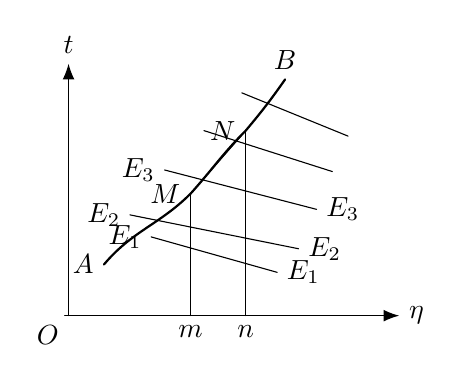
\begin{tikzpicture}[scale=1.0, line cap=round]
\draw[-{Latex[length=2mm]}] (0,0) -- (0,3.2) node[above] {$t$};
\draw[-{Latex[length=2mm]}] (-.05,0) -- (4.2,0) node[right] {$\eta$};
\node[below left] at (0,0) {$O$};
\draw[thick] (.45,.65) node[left] {$A$} to[out=50,in=225] (1.55,1.55) node[left] {$M$} to[out=48,in=225] (2.25,2.35) node[left] {$N$} to[out=50,in=235] (2.75,3.0) node[above] {$B$};
\draw[thin] (1.55,0) node[below] {$m$} -- (1.55,1.55);
\draw[thin] (2.25,0) node[below] {$n$} -- (2.25,2.35);
\draw[thin] (1.55,1.55) -- (2.25,2.35);
\draw[thin] (1.05,1.0) node[left] {$E_1$} -- (2.65,.55) node[right] {$E_1$};
\draw[thin] (.78,1.28) node[left] {$E_2$} -- (2.92,.85) node[right] {$E_2$};
\draw[thin] (1.22,1.85) node[left] {$E_3$} -- (3.15,1.35) node[right] {$E_3$};
\draw[thin] (1.72,2.35) -- (3.35,1.83);
\draw[thin] (2.2,2.83) -- (3.55,2.28);
\figlabel{Fig. 5.}
\end{tikzpicture}
\end{center}


\begin{center}
\bfseries Diagrams in which the Isometrics, Isopiestics, Isothermals, Isodynamics and Isentropics of a Perfect Gas are all Straight Lines.
\end{center}

There are many cases in which it is of more importance that it should be easy to draw the lines of equal volume, pressure, temperature, energy and entropy, than that work and heat should be represented in the simplest manner. In such cases it may be expedient to give up the condition that the scale ($\gamma$) of work and heat shall be constant, when by that means it is possible to gain greater simplicity in the form of the lines just mentioned.

In the case of a perfect gas, the three relations between the quantities $v,p,t,e$ and $\eta$ are given on pages 12, 13, equations (A), (B) and (D). These equations may be easily transformed into the three
\begin{align}
\log p+\log v-\log t&=\log a, \tag{H}\\
\log e-\log t&=\log c, \tag{I}\\
\eta-c\log e-a\log v&=0; \tag{J}
\end{align}
so that the three relations between the quantities $\log v,\log p,\log t,\log e$ and $\eta$ are expressed by linear equations, and it will be possible to make the five systems of lines all rectilinear in the same diagram, the distances of the isometrics being proportional to the differences of the logarithms of the volumes, the distances of the isopiestics being proportional to the differences of the logarithms of the pressures, and so with the isothermals and the isodynamics,--the distances of the isentropics, however, being proportional to the differences of entropy simply.

The scale of work and heat in such a diagram will vary inversely as the temperature. For if we imagine systems of isentropics and isothermals drawn throughout the diagram for equal small differences of entropy and temperature, the isentropics will be equidistant, but the distances of the isothermals will vary inversely as the temperature, and the small quadrilaterals into which the diagram is divided will vary in the same ratio: $\therefore\ \gamma\propto 1/t$. (See p. 5.)

So far, however, the form of the diagram has not been completely defined. This may be done in various ways: e.g., if $x$ and $y$ be the rectangular co-ordinates, we may make
\[
\left\{\begin{array}{l}
x=\log v,\\
y=\log p;
\end{array}\right.
\quad\hbox{or}\quad
\left\{\begin{array}{l}
x=\eta,\\
y=\log t;
\end{array}\right.
\quad\hbox{or}\quad
\left\{\begin{array}{l}
x=\log v,\\
y=\eta;
\end{array}\right.
\quad \hbox{etc.}
\]
Or we may set the condition that the logarithms of volume, of pressure and of temperature, shall be represented in the diagram on the same scale. (The logarithms of energy are necessarily represented on the same scale as those of temperature.) This will require that the isometrics, isopiestics and isothermals cut one another at angles of $60^\circ$.

The general character of all these diagrams, which may be derived from one another by projection by parallel lines, may be illustrated by the case in which $x=\log v$, and $y=\log p$. Through any point $A$ (fig. 6) of such a diagram let there be drawn the isometric $vv'$, the isopiestic $pp'$, the isothermal $tt'$ and the isentropic $\eta\eta'$. The lines $pp'$ and $vv'$ are of course parallel to the axes.


\begin{center}
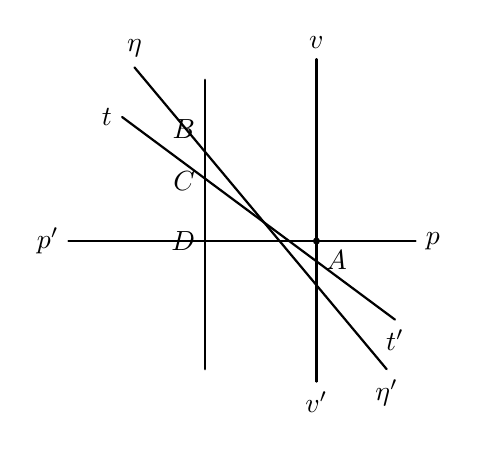
\begin{tikzpicture}[scale=1.05, line cap=round]
\draw[thick] (0,0) -- (4.2,0) node[right] {$p$};
\node[left] at (0,0) {$p'$};
\draw[thick] (3.0,-1.7) -- (3.0,2.2) node[above] {$v$};
\node[below] at (3.0,-1.7) {$v'$};
\coordinate (A) at (3,0);
\coordinate (D) at (1.65,0);
\coordinate (C) at (1.65,.72);
\coordinate (B) at (1.65,1.35);
\draw[thick] (.8,2.1) node[above] {$\eta$} -- (3.85,-1.55) node[below] {$\eta'$};
\draw[thick] (.65,1.5) node[left] {$t$} -- (3.95,-.95) node[below] {$t'$};
\draw[thick] (1.65,-1.55) -- (1.65,1.95);
\draw[fill=black] (A) circle (1pt) node[below right] {$A$};
\node[left] at (D) {$D$};
\node[left] at (C) {$C$};
\node[left] at (B) {$B$};
\figlabel{Fig. 6.}
\end{tikzpicture}
\end{center}


Also by equation (H)
\[
\tan tAp=\left(\frac{dy}{dx}\right)_t
=\left(\frac{d\log p}{d\log v}\right)_t=-1,
\]
and by (G)
\[
\tan\eta Ap=\left(\frac{dy}{dx}\right)_\eta
=\left(\frac{d\log p}{d\log v}\right)_\eta=-\frac{c+a}{c}.
\]
Therefore, if we draw another isometric, cutting $\eta\eta'$, $tt'$, and $pp'$ in $B,C$ and $D$,
\[
\frac{BD}{CD}=\frac{c+a}{c},\qquad
\frac{BC}{CD}=\frac{a}{c},\qquad
\frac{CD}{BC}=\frac{c}{a}.
\]
Hence, in the diagrams of different gases, $CD\div BC$ will be proportional to the specific heat determined for equal volumes and for constant volume.

As the specific heat, thus determined, has probably the same value for most simple gases, the isentropics will have the same inclination in diagrams of this kind for most simple gases. This inclination may easily be found by a method which is independent of any units of measurement, for
\[
BD:CD::\left(\frac{d\log p}{d\log v}\right)_\eta :
\left(\frac{d\log p}{d\log v}\right)_t ::
\left(\frac{dp}{dv}\right)_\eta :
\left(\frac{dp}{dv}\right)_t ,
\]
i.e., $BD\div CD$ is equal to the quotient of the co-efficient of elasticity under the condition of no transmission of heat, divided by the co-efficient of elasticity at constant temperature. This quotient for a simple gas is generally given as $1.408$ or $1.421$. As
\[
CA\div CD=\sqrt{2}=1.414,
\]
$BD$ is very nearly equal to $CA$ (for simple gases), which relation it may be convenient to use in the construction of the diagram.

In regard to compound gases the rule seems to be, that the specific heat (determined for equal volumes and for constant volume) is to the specific heat of a simple gas inversely as the volume of the compound is to the volume of its constituents (in the condition of gas); that is, the value of $BC\div CD$ for a compound gas is to the value of $BC\div CD$ for a simple gas, as the volume of the compound is to the volume of its constituents. Therefore, if we compare the diagrams (formed by this method) for a simple and a compound gas, the distance $DA$ and therefore $CD$ being the same in each, $BC$ in the diagram of the compound gas will be to $BC$ in the diagram of the simple gas as the volume of the compound is to the volume of its constituents.

Although the inclination of the isentropics is independent of the quantity of gas under consideration, the rate of increase of $\eta$ will vary with this quantity. In regard to the rate of increase of $t$, it is evident that if the whole diagram be divided into squares by isopiestics and isometrics drawn at equal distances, and isothermals be drawn as diagonals to these squares, the volumes of the isometrics, the pressures of the isopiestics and the temperatures of the isothermals will each form a geometrical series, and in all these series the ratio of two contiguous terms will be the same.

The properties of the diagrams obtained by the other methods mentioned on page 17 do not differ essentially from those just described. For example, in any such diagram, if through any point we draw an isentropic, an isothermal and an isopiestic, which cut any isometric not passing through the same point, the ratio of the segments of the isometric will have the value which has been found for $BC:CD$.

In treating the case of vapors also, it may be convenient to use diagrams in which $x=\log v$ and $y=\log p$, or in which $x=\eta$ and $y=\log t$; but the diagrams formed by these methods will evidently be radically different from one another. It is to be observed that each of these methods is what may be called a \emph{method of definite scale} for work and heat; that is, the value of $\gamma$ in any part of the diagram is independent of the properties of the fluid considered. In the first method
\[
\gamma=\frac{1}{e^{x+y}},
\]
in the second
\[
\gamma=\frac{1}{e^y}.
\]
In this respect these methods have an advantage over many others. For example, if we should make $x=\log v$, $y=\eta$, the value of $\gamma$ in any part of the diagram would depend upon the properties of the fluid, and would probably not vary in any case, except that of a perfect gas, according to any simple law.

The conveniences of the entropy-temperature method will be found to belong in nearly the same degree to the method in which the co-ordinates are equal to the entropy and the logarithm of the temperature. No serious difficulty attaches to the estimation of heat and work in a diagram formed on the latter method on account of the variation of the scale on which they are represented, as this variation follows so simple a law. It may often be of use to remember that such a diagram may be reduced to an entropy-temperature diagram by a vertical compression or extension, such that the distances of the isothermals shall be made proportional to their differences of temperature. Thus if we wish to estimate the work or heat of the circuit $ABCD$ (fig. 7), we may draw a number of equidistant ordinates (isentropics) as if to estimate the included area, and for each of the ordinates take the differences of temperature of the points where it cuts the circuit; these differences of temperature will be equal to the lengths of the segments made by the corresponding circuit in the entropy-temperature diagram upon a corresponding system of equidistant ordinates, and may be used to calculate the area of the circuit in the entropy-temperature diagram, i.e., to find the work or heat required.


\begin{center}
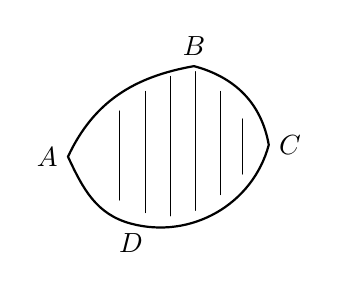
\begin{tikzpicture}[scale=1.0, line cap=round]
\draw[thick] (0.2,1.0) node[left] {$A$}
  to[out=65,in=190] (1.8,2.15) node[above] {$B$}
  to[out=-15,in=100] (2.75,1.15) node[right] {$C$}
  to[out=-105,in=-15] (1.0,.15) node[below] {$D$}
  to[out=165,in=-65] cycle;
\foreach \x/\ya/\yb in {0.85/0.45/1.58,1.18/0.29/1.83,1.50/0.25/2.02,1.82/0.32/2.08,2.14/0.52/1.83,2.42/0.78/1.48}{
  \draw[thin] (\x,\ya) -- (\x,\yb);
}
\figlabel{Fig. 7.}
\end{tikzpicture}
\end{center}


We may find the work of any path by applying the same process to the circuit formed by the path, the isometric of the final state, the line of no pressure (or any isopiestic; see note on page 9), and the isometric of the initial state. And we may find the heat of any path by applying the same process to a circuit formed by the path, the ordinates of the extreme points and the line of absolute cold. That this line is at an infinite distance occasions no difficulty. The lengths of the ordinates in the entropy-temperature diagram which we desire are given by the temperature of points in the path determined (in either diagram) by equidistant ordinates.

The properties of the part of the entropy-temperature diagram representing a mixture of vapor and liquid, which are given on page 14, will evidently not be altered if the ordinates are made proportional to the logarithms of the temperatures instead of the temperatures simply.

The representation of specific heat in the diagram under discussion is peculiarly simple. The specific heat of any substance at constant volume or under constant pressure may be defined as the value of
\[
\left(\frac{dH}{dt}\right)_v
\quad\hbox{or}\quad
\left(\frac{dH}{dt}\right)_p,
\quad\hbox{i.e.,}\quad
\left(\frac{d\eta}{d\log t}\right)_v
\quad\hbox{or}\quad
\left(\frac{d\eta}{d\log t}\right)_p,
\]
for a certain quantity of the substance. Therefore, if we draw a diagram, in which $x=\eta$ and $y=\log t$, for that quantity of the substance which is used for the determination of the specific heat, the tangents of the angles made by the isometrics and the isopiestics with the ordinates in the diagram will be equal to the specific heat of the substance determined for constant volume and for constant pressure respectively. Sometimes, instead of the condition of constant volume or constant pressure, some other condition is used in the determination of specific heat. In all cases, the condition will be represented by a line in the diagram, and the tangent of the angle made by this line with an ordinate will be equal to the specific heat as thus defined. If the diagram be drawn for any other quantity of the substance, the specific heat for constant volume or constant pressure, or for any other condition, will be equal to the tangent of the proper angle in the diagram, multiplied by the ratio of the quantity of the substance for which the specific heat is determined to the quantity for which the diagram is drawn.\footnote{From this general property of the diagram, its character in the case of a perfect gas might be immediately deduced.}

\begin{center}
\bfseries The Volume-entropy Diagram.
\end{center}

The method of representation, in which the co-ordinates of the point in the diagram are made equal to the volume and entropy of the body, presents certain characteristics which entitle it to a somewhat detailed consideration, and for some purposes give it substantial advantages over any other method. We might anticipate some of these advantages from the simple and symmetrical form of the general equations of thermodynamics, when volume and entropy are chosen as independent variables, viz.:--\footnote{See page 2, equations (2), (3) and (4). In general, in this article, where differential coefficients are used, the quantity which is constant in the differentiation is indicated by a subscript letter. In this discussion of the volume-entropy diagram, however, $v$ and $\eta$ are uniformly regarded as the independent variables, and the subscript letter is omitted.}


\[
p=-\frac{de}{dv}, \tag{11}
\]
\[
t=\frac{de}{d\eta}. \tag{12}
\]
\[
dW=p\,dv,\qquad dH=t\,d\eta.
\]
Eliminating $p$ and $t$ we have also
\[
dW=-\frac{de}{dv}\,dv, \tag{13}
\]
\[
dH=\frac{de}{d\eta}\,d\eta. \tag{14}
\]

The geometrical relations corresponding to these equations are in the volume-entropy diagram extremely simple. To fix our ideas, let the axes of volume and entropy be horizontal and vertical respectively, volume increasing toward the right and entropy upward. Then the pressure taken negatively will equal the ratio of the difference of energy to the difference of volume of two adjacent points in the same horizontal line, and the temperature will equal the ratio of the difference of energy to the difference of entropy of two adjacent points in the same vertical line. Or, if a series of isodynamics be drawn for equal infinitesimal differences of energy, any series of horizontal lines will be divided into segments inversely proportional to the pressure, and any series of vertical lines into segments inversely proportional to the temperature. We see by equations (13) and (14), that for a motion parallel to the axis of volume, the heat received is 0, and the work done is equal to the decrease of the energy, while for a motion parallel to the axis of entropy, the work done is 0, and the heat received is equal to the increase of the energy. These two propositions are true either for elementary paths or for those of finite length. In general, the work for any element of a path is equal to the product of the pressure in that part of the diagram into the horizontal projection of the element of the path, and the heat received is equal to the product of the temperature into the vertical projection of the element of the path.

If we wish to estimate the value of the integrals $\int p\,dv$ and $\int t\,d\eta$, which represent the work and heat of any path, by means of measurements upon the diagram, or if we wish to appreciate readily by the eye the approximate value of these expressions, or if we merely wish to illustrate their meaning by means of the diagram; for any of these purposes the diagram which we are now considering will have the advantage that it represents the differentials $dv$ and $d\eta$ more simply and clearly than any other.

But we may also estimate the work and heat of any path by means of an integration extending over the elements of an area, viz.: by the formulae of page 7,
\begin{align*}
W^C=H^C&=\Sigma^C \frac{1}{\gamma}\,\delta A,\\
W^S&=\Sigma^{[S,v'',p^0,v']}\frac{1}{\gamma}\,\delta A,\\
H^S&=\Sigma^{[S,\eta'',t^0,\eta']}\frac{1}{\gamma}\,\delta A.
\end{align*}
In regard to the limits of integration in these formulae, we see that for the work of any path which is not a circuit, the bounding line is composed of the path, the line of no pressure and two vertical lines, and for the heat of the path, the bounding line is composed of the path, the line of absolute cold and two horizontal lines.

As the sign of $\gamma$, as well as that of $\delta A$, will be indeterminate until we decide in which direction an area must be circumscribed in order to be considered positive, we will call an area positive which is circumscribed in the direction in which the hands of a watch move. This choice, with the positions of the axes of volume and entropy which we have supposed, will make the value of $\gamma$ in most cases positive, as we shall see hereafter.

The value of $\gamma$, in a diagram drawn according to this method, will depend upon the properties of the body for which the diagram is drawn. In this respect, this method differs from all the others which have been discussed in detail in this article. It is easy to find an expression for $\gamma$ depending simply upon the variations of the energy, by comparing the area and the work or heat of an infinitely small circuit in the form of a rectangle having its sides parallel to the two axes.

\begin{figure}[h]
\centering
\begin{tikzpicture}[scale=1.0,line cap=round]
\draw[-{Latex[length=2mm]}] (0,0)--(0,2.45) node[above] {$\eta$};
\draw[-{Latex[length=2mm]}] (0,0)--(3.3,0) node[right] {$v$};
\node[below left] at (0,0) {$O$};
\draw[thick] (1.45,1.10) rectangle (1.86,1.43);
\node[left] at (1.45,1.43) {$N_1$};
\node[right] at (1.86,1.43) {$N_2$};
\node[right] at (1.86,1.10) {$N_3$};
\node[left] at (1.45,1.10) {$N_4$};
\node at ($(current bounding box.south)+(0,-0.28)$) {\small Fig. 8.};
\end{tikzpicture}
\end{figure}

Let $N_1N_2N_3N_4$ (fig. 8) be such a circuit, and let it be described in the order of the numerals, so that the area is positive. Also let $e_1,e_2,e_3,e_4$ represent the energy at the four corners. The work done in the four sides in order commencing at $N_1$, will be $e_1-e_2,0,e_3-e_4,0$. The total work, therefore, for the rectangular circuit is
\[
e_1-e_2+e_3-e_4.
\]
Now as the rectangle is infinitely small, if we call its sides $dv$ and $d\eta$, the above expression will be equivalent to
\[
-\frac{d^2e}{dv\,d\eta}\,dv\,d\eta.
\]
Dividing by the area $dv\,d\eta$, and writing $\gamma_{v,\eta}$ for the scale of work and heat in a diagram of this kind, we have
\[
\frac{1}{\gamma_{v,\eta}}
=-\frac{d^2e}{dv\,d\eta}=\frac{dp}{d\eta}=-\frac{dt}{dv}. \tag{15}
\]
The two last expressions for the value of $1\div\gamma_{v,\eta}$ indicate that the value of $\gamma_{v,\eta}$ in different parts of the diagram will be indicated proportionally by the segments into which vertical lines are divided by a system of equidifferent isopiestics, and also by the segments into which horizontal lines are divided by a system of equidifferent isothermals. These results might also be derived directly from the propositions on page 5.

As, in almost all cases, the pressure of a body is increased when it receives heat without change of volume, $dp/d\eta$ is in general positive, and the same will be true of $\gamma_{v,\eta}$ under the assumptions which we have made in regard to the directions of the axes (page 21) and the definition of a positive area (page 22).

In the estimation of work and heat it may often be of use to consider the deformation necessary to reduce the diagram to one of constant scale for work and heat. Now if the diagram be so deformed that each point remains in the same vertical line, but moves in this line so that all isopiestics become straight and horizontal lines at distances proportional to their differences of pressure, it will evidently become a volume-pressure diagram. Again, if the diagram be so deformed that each point remains in the same horizontal line, but moves in it so that isothermals become straight and vertical lines at distances proportional to their differences of temperature, it will become an entropy-temperature diagram. These considerations will enable us to compute numerically the work or heat of any path which is given in a volume-entropy diagram, when the pressure and temperature are known for all points of the path, in a manner analogous to that explained on page 19.

The ratio of any element of area in the volume-pressure or the entropy-temperature diagram, or in any other in which the scale of work and heat is unity, to the corresponding element in the volume-entropy diagram is represented by $1/\gamma_{v,\eta}$ or $-d^2e/(dv\,d\eta)$. The cases in which this ratio is 0, or changes its sign, demand especial attention, as in such cases the diagrams of constant scale fail to give a satisfactory representation of the properties of the body, while no difficulty or inconvenience arises in the use of the volume-entropy diagram.

As $-d^2e/(dv\,d\eta)=dp/d\eta$, its value is evidently zero in that part of the diagram which represents the body when in part solid, in part liquid, and in part vapor. The properties of such a mixture are very simply and clearly exhibited in the volume-entropy diagram.

Let the temperature and the pressure of the mixture, which are independent of the proportions of vapor, solid and liquid, be denoted by $t'$ and $p'$. Also let $V,L$ and $S$ (fig. 9) be points of the diagram which indicate the volume and entropy of the body in three perfectly defined states, viz.: that of a vapor of temperature $t'$ and pressure $p'$, that of a liquid of the same temperature and pressure, and that of a solid of the same temperature and pressure. And let $v_V,\eta_V,v_L,\eta_L,v_S,\eta_S$ denote the volume and entropy of these states. The position of the point which represents the body, when part is vapor, part liquid, and part solid, these parts being as $\mu,\nu$, and $1-\mu-\nu$, is determined by the equations
\begin{align*}
v&=\mu v_V+\nu v_L+(1-\mu-\nu)v_S,\\
\eta&=\mu\eta_V+\nu\eta_L+(1-\mu-\nu)\eta_S,
\end{align*}
where $v$ and $\eta$ are the volume and entropy of the mixture. The truth of the first equation is evident. The second may be written
\[
\eta-\eta_S=\mu(\eta_V-\eta_S)+\nu(\eta_L-\eta_S),
\]
or multiplying by $t'$,
\[
t'(\eta-\eta_S)=\mu t'(\eta_V-\eta_S)+\nu t'(\eta_L-\eta_S).
\]
The first member of this equation denotes the heat necessary to bring the body from the state $S$ to the state of the mixture in question under the constant temperature $t'$, while the terms of the second member denote separately the heat necessary to vaporize the part $\mu$, and to liquefy the part $\nu$ of the body.

\begin{figure}[h]
\centering
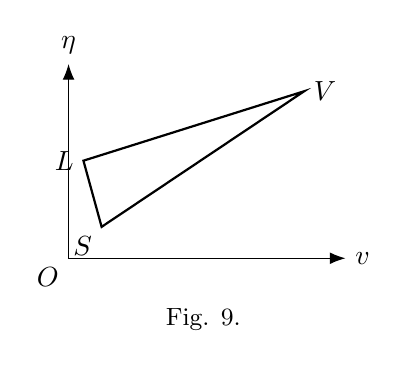
\begin{tikzpicture}[scale=1.05,line cap=round]
\draw[-{Latex[length=2mm]}] (0,0)--(0,2.35) node[above] {$\eta$};
\draw[-{Latex[length=2mm]}] (0,0)--(3.35,0) node[right] {$v$};
\node[below left] at (0,0) {$O$};
\coordinate (S) at (.40,.38);\coordinate (L) at (.18,1.18);\coordinate (V) at (2.85,2.02);
\draw[thick] (S)--(L)--(V)--cycle;
\node[left] at (L) {$L$};\node[below left] at (S) {$S$};\node[right] at (V) {$V$};
\node at ($(current bounding box.south)+(0,-0.28)$) {\small Fig. 9.};
\end{tikzpicture}
\end{figure}

The values of $v$ and $\eta$ are such as would give the center of gravity of masses $\mu,\nu$ and $1-\mu-\nu$ placed at the points $V,L$ and $S$.\footnote{These points will not be in the same straight line unless
\[
t'(\eta_V-\eta_S):t'(\eta_L-\eta_S)::v_V-v_S:v_L-v_S,
\]
a condition very unlikely to be fulfilled by any substance. The first and second terms of this proportion denote the heat of vaporization (from the solid state) and that of liquefaction.} Hence the part of the diagram which represents a mixture of vapor, liquid and solid, is the triangle $VLS$. The pressure and temperature are constant for this triangle, i.e., an isopiestic and also an isothermal here expand to cover a space. The isodynamics are straight and equidistant for equal differences of energy. For $de/dv=-p'$ and $de/d\eta=t'$, both of which are constant throughout the triangle.

This case can be but very imperfectly represented in the volume-pressure, or in the entropy-temperature diagram. For all points in the same vertical line in the triangle $VLS$ will, in the volume-pressure diagram, be represented by a single point, as having the same volume and pressure. And all the points in the same horizontal line will be represented in the entropy-temperature diagram by a single point, as having the same entropy and temperature. In either diagram, the whole triangle reduces to a straight line. It must reduce to a line in any diagram whatever of constant scale, as its area must become 0 in such a diagram. This must be regarded as a defect in these diagrams, as essentially different states are represented by the same point. In consequence, any circuit within the triangle $VLS$ will be represented in any diagram of constant scale by two paths of opposite directions superposed, the appearance being as if a body should change its state and then return to its original state by inverse processes, so as to repass through the same series of states. It is true that the circuit in question is like this combination of processes in one important particular, viz.: that $W=H=0$, i.e., there is no transformation of heat into work. But this very fact, that a circuit without transformation of heat into work is possible, is worthy of distinct representation.

A body may have such properties that in one part of the volume-entropy diagram $1/\gamma_{v,\eta}$, i.e., $dp/d\eta$ is positive, and in another negative. These parts of the diagram may be separated by a line, in which $dp/d\eta=0$, or by one in which $dp/d\eta$ changes abruptly from a positive to a negative value.\footnote{The line which represents the various states of water at its maximum density for various constant pressures is an example of the first case. A substance which as a liquid has no proper maximum density for constant pressure, but which expands in solidifying, affords an example of the second case.} (In part, also, they may be separated by an area in which $dp/d\eta=0$.) In the representation of such cases in any diagram of constant scale, we meet with a difficulty of the following nature.

\begin{figure}[h]
\centering
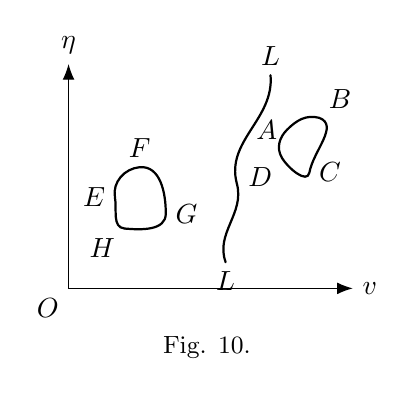
\begin{tikzpicture}[scale=.95,line cap=round]
\draw[-{Latex[length=2mm]}] (0,0)--(0,3.0) node[above] {$\eta$};
\draw[-{Latex[length=2mm]}] (0,0)--(3.8,0) node[right] {$v$};
\node[below left] at (0,0) {$O$};
\draw[thick] (2.1,.35) to[out=110,in=-75] (2.25,1.4) to[out=105,in=-85] (2.7,2.85);
\node[below] at (2.1,.35) {$L$};\node[above] at (2.7,2.85) {$L$};
\draw[thick] (.75,.8) to[out=-5,in=-90] (1.3,1.0) to[out=90,in=5] (.95,1.62) to[out=185,in=100] (.62,1.22) to[out=-80,in=175] cycle;
\node[left] at (.62,1.22) {$E$};\node[above] at (.95,1.62) {$F$};\node[right] at (1.3,1.0) {$G$};\node[below left] at (.75,.8) {$H$};
\draw[thick] (2.85,1.75) to[out=-60,in=-100] (3.22,1.55) to[out=80,in=-20] (3.35,2.28) to[out=165,in=45] (2.92,2.12) to[out=-135,in=120] cycle;
\node[left] at (2.92,2.12) {$A$};\node[above right] at (3.35,2.28) {$B$};\node[right] at (3.22,1.55) {$C$};\node[below left] at (2.85,1.75) {$D$};
\node at ($(current bounding box.south)+(0,-0.28)$) {\small Fig. 10.};
\end{tikzpicture}
\end{figure}

Let us suppose that on the right of the line $LL$ (fig. 10) in a volume-entropy diagram, $dp/d\eta$ is positive, and on the left negative. Then, if we draw any circuit $ABCD$ on the right side of $LL$, the direction being that of the hands of a watch, the work and heat of the circuit will be positive. But if we draw any circuit $EFGH$ in the same direction on the other side of the line $LL$, the work and heat will be negative. For
\[
W=H=\Sigma\frac{1}{\gamma_{v,\eta}}\,\delta A
=\Sigma\frac{dp}{d\eta}\,\delta A,
\]
and the direction of the circuits makes the areas positive in both cases. Now if we should change this diagram into any diagram of constant scale, the areas of the circuits, as representing proportionally the work done in each case, must necessarily have opposite signs, i.e., the direction of the circuits must be opposite. We will suppose that the work done is positive in the diagram of constant scale, when the direction of the circuit is that of the hands of a watch. Then, in that diagram, the circuit $ABCD$ would have that direction, and the circuit $EFGH$ the contrary direction, as in figure 11. Now if we imagine an indefinite number of circuits on each side of $LL$ in the volume-entropy diagram, it will be evident that to transform such a diagram into one of constant scale, so as to change the direction of all the circuits on one side of $LL$, and of none on the other the diagram must be folded over along that line; so that the points on one side of $LL$ in a diagram of constant scale do not represent any states of the body, while on the other side of this line, each point, for a certain distance at least, represents two different states of the body, which in the volume-entropy diagram are represented by points on opposite sides of the line $LL$. We have thus in a part of the field two diagrams superposed, which must be carefully distinguished. If this be done, as by the help of different colors, or of continuous and dotted lines, or otherwise, and it is remembered that there is no continuity between these superposed diagrams, except along the bounding line $LL$, all the general theorems which have been developed in this article can be readily applied to the diagram. But to the eye or to the imagination, the figure will necessarily be much more confusing than a volume-entropy diagram.

\begin{figure}[h]
\centering
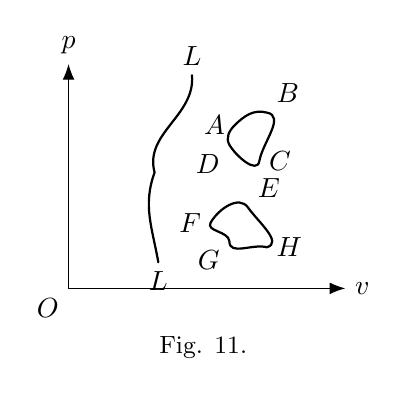
\begin{tikzpicture}[scale=.95,line cap=round]
\draw[-{Latex[length=2mm]}] (0,0)--(0,3.0) node[above] {$p$};
\draw[-{Latex[length=2mm]}] (0,0)--(3.7,0) node[right] {$v$};
\node[below left] at (0,0) {$O$};
\draw[thick] (1.2,.35) to[out=100,in=-110] (1.15,1.55) to[out=105,in=-85] (1.65,2.85);
\node[below] at (1.2,.35) {$L$};\node[above] at (1.65,2.85) {$L$};
\draw[thick] (2.15,1.92) to[out=-60,in=-100] (2.55,1.70) to[out=80,in=-10] (2.65,2.35) to[out=165,in=45] (2.22,2.18) to[out=-135,in=120] cycle;
\node[left] at (2.22,2.18) {$A$};\node[above right] at (2.65,2.35) {$B$};\node[right] at (2.55,1.70) {$C$};\node[below left] at (2.15,1.92) {$D$};
\draw[thick] (1.90,.88) to[out=60,in=125] (2.40,1.08) to[out=-55,in=15] (2.65,.55) to[out=165,in=-90] (2.15,.63) to[out=95,in=-120] cycle;
\node[left] at (1.90,.88) {$F$};\node[above right] at (2.40,1.08) {$E$};\node[right] at (2.65,.55) {$H$};\node[below left] at (2.15,.63) {$G$};
\node at ($(current bounding box.south)+(0,-0.28)$) {\small Fig. 11.};
\end{tikzpicture}
\end{figure}

If $dp/d\eta=0$ for the line $LL$, there will be another inconvenience in the use of any diagram of constant scale, viz.: in the vicinity of the line $LL$, $dp/d\eta$, i.e., $1\div\gamma_{v,\eta}$ will have a very small value, so that areas will be very greatly reduced in the diagram of constant scale, as compared with the corresponding areas in the volume-entropy diagram. Therefore, in the former diagram, either the isometrics, or the isentropics, or both, will be crowded together in the vicinity of the line $LL$, so that this part of the diagram will be necessarily indistinct.

It may occur, however, in the volume-entropy diagram, that the same point must represent two different states of the body. This occurs in the case of liquids which can be vaporized. Let $MM$ (fig. 12) be the line representing the states of the liquid bordering upon vaporization. This line will be near to the axis of entropy, and nearly parallel to it. If the body is in a state represented by a point of the line $MM$, and is compressed without addition or subtraction of heat, it will remain of course liquid. Hence, the points of the space immediately on the left of $MM$ represent simple liquid. On the other hand, the body being in the original state, if its volume should be increased without addition or subtraction of heat, and if the conditions necessary for vaporization are present (conditions relative to the body enclosing the liquid in question, etc.), the liquid will become partially vaporized, but if these conditions are not present, it will continue liquid. Hence, every point on the right of $MM$ and sufficiently near to it represents two different states of the body, in one of which it is partially vaporized, and in the other it is entirely liquid. If we take the points as representing the mixture of vapor and liquid, they form one diagram, and if we take them as representing simple liquid, they form a totally different diagram superposed on the first. There is evidently no continuity between these diagrams except at the line $MM$; we may regard them as upon separate sheets united only along $MM$. For the body cannot pass from the state of partial vaporization to the state of liquid except at this line. The reverse process is indeed possible; the body can pass from the state of superheated liquid to that of partial vaporization, if the conditions of vaporization alluded to above are supplied, or if the increase of volume is carried beyond a certain limit, but not by gradual changes or reversible processes. After such a change, the point representing the state of the body will be found in a different position from that which it occupied before, but the change of state cannot be properly represented by any path, as during the change the body does not satisfy that condition of uniform temperature and pressure which has been assumed throughout this article, and which is necessary for the graphical methods under discussion. (See note on page 1.)

\begin{figure}[h]
\centering
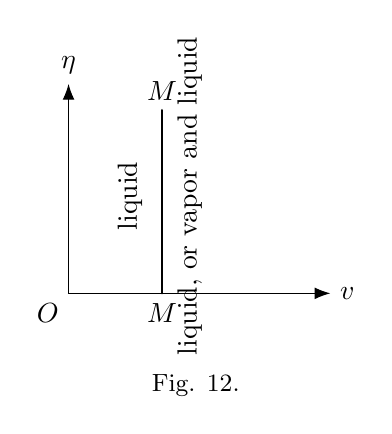
\begin{tikzpicture}[scale=.95,line cap=round]
\draw[-{Latex[length=2mm]}] (0,0)--(0,2.8) node[above] {$\eta$};
\draw[-{Latex[length=2mm]}] (0,0)--(3.5,0) node[right] {$v$};
\node[below left] at (0,0) {$O$};
\draw[thick] (1.25,0)--(1.25,2.45);
\node[below] at (1.25,0) {$M$};\node[above] at (1.25,2.45) {$M$};
\node[rotate=90] at (.82,1.30) {liquid};
\node[rotate=90] at (1.62,1.30) {liquid, or vapor and liquid};
\node at ($(current bounding box.south)+(0,-0.28)$) {\small Fig. 12.};
\end{tikzpicture}
\end{figure}

Of the two superposed diagrams, that which represents simple liquid is a continuation of the diagram on the left of $MM$. The isopiestics, isothermals and isodynamics pass from one to the other without abrupt change of direction or curvature. But that which represents a mixture of vapor and liquid will be different in its character, and its isopiestics and isothermals will make angles in general with the corresponding lines in the diagram of simple liquid. The isodynamics of the diagram of the mixture, and those of the diagram of simple liquid, will differ in general in curvature at the line $MM$, but not in direction, for $de/dv=-p$ and $de/d\eta=t$.

The case is essentially the same with some substances, as water, for example, about the line which separates the simple liquid from a mixture of liquid and solid.

In these cases the inconvenience of having one diagram superposed upon another cannot be obviated by any change of the principle on which the diagram is based. For no distortion can bring the three sheets, which are united along the line $MM$ (one on the left and two on the right), into a single plane surface without superposition. Such cases, therefore, are radically distinguished from those in which the superposition is caused by an unsuitable method of representation.

To find the character of a volume-entropy diagram of a perfect gas, we may make $e$ constant in equation (D) on page 13, which will give for the equation of an isodynamic and isothermal
\[
\eta=a\log v+\mathrm{Const.},
\]
and we may make $p$ constant in equation (G), which will give for the equation of an isopiestic
\[
\eta=(a+c)\log v+\mathrm{Const.}
\]
It will be observed that all the isodynamics and isothermals can be drawn by a single pattern and so also with the isopiestics.

The case will be nearly the same with vapors in a part of the diagram. In that part of the diagram which represents a mixture of liquid and vapor, the isothermals, which of course are identical with the isopiestics, are straight lines. For when a body is vaporized under constant pressure and temperature, the quantities of heat received are proportional to the increments of volume; therefore, the increments of entropy are proportional to the increments of volume. As $de/dv=-p$ and $de/d\eta=t$, any isothermal is cut at the same angle by all the isodynamics, and is divided into equal segments by equidifferent isodynamics. The latter property is useful in drawing systems of equidifferent isodynamics.

\begin{center}
\bfseries Arrangement of the Isometric, Isopiestic, Isothermal and\\ Isentropic about a Point.
\end{center}

The arrangement of the isometric, the isopiestic, the isothermal and the isentropic drawn through any same point, in respect to the order in which they succeed one another around that point, and in respect to the sides of these lines toward which the volume, pressure, temperature and entropy increase, is not altered by any deformation of the surface on which the diagram is drawn, and is therefore independent of the method by which the diagram is formed.\footnote{It is here assumed that, in the vicinity of the point in question, each point in the diagram represents only one state of the body. The propositions developed in the following pages cannot be applied to points of the line where two superposed diagrams are united (see pages 25--28) without certain modifications.} This arrangement is determined by certain of the most characteristic thermodynamic properties of the body in the state in question, and serves in turn to indicate these properties. It is determined, namely, by the value of $\left(dp/d\eta\right)_v$ as positive, negative, or zero, i.e., by the effect of heat as increasing or diminishing the pressure when the volume is maintained constant, and by the nature of the internal thermodynamic equilibrium of the body as stable or neutral,--an unstable equilibrium, except as a matter of speculation, is of course out of the question.

Let us first examine the case in which $\left(dp/d\eta\right)_v$ is positive and the equilibrium is stable. As $\left(dp/d\eta\right)_v$ does not vanish at the point in question, there is a definite isopiestic passing through that point, on one side of which the pressures are greater, and on the other less, than on the line itself. As $\left(dt/dv\right)_\eta=-\left(dp/d\eta\right)_v$, the case is the same with the isothermal. It will be convenient to distinguish the sides of the isometric, isopiestic, etc., on which the volume, pressure, etc., increase, as the positive sides of these lines. The condition of stability requires that, when the pressure is constant, the temperature shall increase with the heat received,--therefore with the entropy. This may be written $[dt:d\eta]_p>0$.\footnote{As the notation $dt/d\eta$ is used to denote the limit of the ratio of $dt$ to $d\eta$, it would not be quite accurate to say that the condition of stability requires that $\left(dt/d\eta\right)_p>0$. This condition requires that the ratio of the differences of temperature and entropy between the point in question and any other infinitely near to it and upon the same isopiestic should be positive. It is not necessary that the limit of this ratio should be positive.} It also requires that, when there is no transmission of heat, the pressure should increase as the volume diminishes, i.e., that $[dp:dv]_\eta<0$. Through the point in question, $A$ (fig. 13), let there be drawn the isometric $vv'$ and the isentropic $\eta\eta'$, and let the positive sides of these lines be indicated as in the figure. The conditions $\left(dp/d\eta\right)_v>0$ and $[dp:dv]_\eta<0$ require that the pressure at $v$ and at $\eta$ shall be greater than at $A$, and hence, that the isopiestic shall fall as $pp'$ in the figure, and have its positive side turned as indicated. Again, the conditions $\left(dt/dv\right)_\eta<0$ and $[dt:d\eta]_p>0$ require that the temperature at $\eta$ and at $p$ shall be greater than at $A$, and hence, that the isothermal shall fall as $tt'$ and have its positive side turned as indicated. As it is not necessary that $\left(dt/d\eta\right)_p>0$, the lines $pp'$ and $tt'$ may be tangent to one another at $A$, provided that they cross one another, so as to have the same order about the point $A$ as is represented in the figure; i.e., they may have a contact of the second (or any even) order.\footnote{An example of this is doubtless to be found at the critical point of a fluid. See Dr. Andrews ``On the continuity of the gaseous and liquid states of matter.'' \emph{Phil. Trans.}, vol. 159, p. 575. If the isothermal and isopiestic have a simple tangency at $A$, on one side of that point they will have such directions as will express an unstable equilibrium. A line drawn through all such points in the diagram will form a boundary to the possible part of the diagram. It may be that the part of the diagram of a fluid, which represents the superheated liquid state, is bounded on one side by such a line.} But the condition that $\left(dp/d\eta\right)_v>0$, and hence $\left(dt/dv\right)_\eta<0$, does not allow $pp'$ to be tangent to $vv'$, nor $tt'$ to $\eta\eta'$.

\begin{figure}[h]
\centering
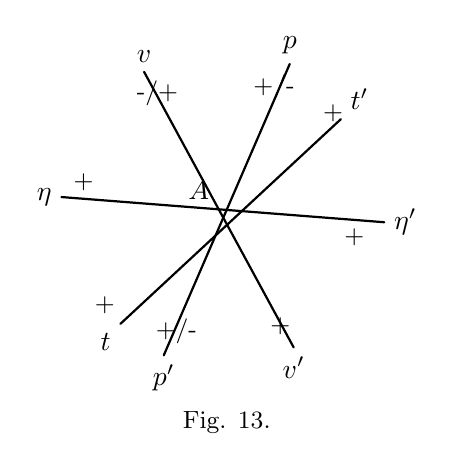
\begin{tikzpicture}[scale=1.0,line cap=round]
\coordinate (A) at (0,0);\node[above left] at (A) {$A$};
\draw[thick] (-2.0,.16)--(2.1,-.16);\node[left] at (-2.0,.16) {$\eta$};\node[right] at (2.1,-.16) {$\eta'$};
\draw[thick] (-1.25,-1.45)--(1.55,1.15);\node[below left] at (-1.25,-1.45) {$t$};\node[above right] at (1.55,1.15) {$t'$};
\draw[thick] (-.95,1.75)--(.95,-1.75);\node[above] at (-.95,1.75) {$v$};\node[below] at (.95,-1.75) {$v'$};
\draw[thick] (-.70,-1.85)--(.90,1.85);\node[below] at (-.70,-1.85) {$p'$};\node[above] at (.90,1.85) {$p$};
\foreach \x/\y/\s in {-1.72/.35/{+},1.72/-.35/{+},-1.45/-1.22/{+},1.45/1.22/{+},-.78/1.48/{-/+},.78/-1.48/{+},-.54/-1.55/{+/-},.70/1.55/{+/-}}{\node at (\x,\y) {\small \s};}
\node at ($(current bounding box.south)+(0,-0.28)$) {\small Fig. 13.};
\end{tikzpicture}
\end{figure}

If $\left(dp/d\eta\right)_v$ be still positive, but the equilibrium be neutral, it will be possible for the body to change its state without change either of temperature or of pressure; i.e., the isothermal and isopiestic will be identical. The lines will fall as in figure 13, except that the isothermal and isopiestic will be superposed.

In like manner, if $\left(dp/d\eta\right)_v<0$, it may be proved that the lines will fall as in figure 14 for stable equilibrium, and in the same way for neutral equilibrium, except that $pp'$ and $tt'$ will be superposed.\footnote{When it is said that the arrangement of the lines in the diagram must be like that in figure 13 or in figure 14, it is not meant to exclude the case in which the figure (13 or 14) must be turned over, in order to correspond with the diagram. In the case, however, of diagrams formed by any of the methods mentioned in this article, if the directions of the axes be such as we have assumed, the agreement with figure 13 will be without inversion, and the agreement with fig. 14 will also be without inversion for volume-entropy diagrams, but with inversion for volume-pressure or entropy-temperature diagrams, or those in which $x=\log v$ and $y=\log p$, or $x=\eta$ and $y=\log t$.}

\begin{figure}[h]
\centering
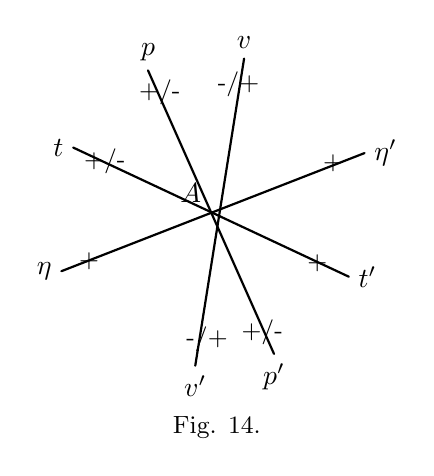
\begin{tikzpicture}[scale=1.0,line cap=round]
\coordinate (A) at (0,0);\node[above left] at (A) {$A$};
\draw[thick] (-1.9,-.75)--(1.95,.75);\node[left] at (-1.9,-.75) {$\eta$};\node[right] at (1.95,.75) {$\eta'$};
\draw[thick] (-1.75,.82)--(1.75,-.82);\node[left] at (-1.75,.82) {$t$};\node[right] at (1.75,-.82) {$t'$};
\draw[thick] (-.80,1.80)--(.80,-1.80);\node[above] at (-.80,1.80) {$p$};\node[below] at (.80,-1.80) {$p'$};
\draw[thick] (-.20,-1.95)--(.42,1.95);\node[below] at (-.20,-1.95) {$v'$};\node[above] at (.42,1.95) {$v$};
\foreach \x/\y/\s in {-1.55/-.62/{+},1.55/.62/{+},-1.35/.65/{+/-},1.35/-.65/{+},-.65/1.52/{+/-},.65/-1.52/{+/-},-.05/-1.62/{-/+},.35/1.62/{-/+}}{\node at (\x,\y) {\small \s};}
\node at ($(current bounding box.south)+(0,-0.28)$) {\small Fig. 14.};
\end{tikzpicture}
\end{figure}

The case that $\left(dp/d\eta\right)_v=0$ includes a considerable number of conceivable cases, which would require to be distinguished. It will be sufficient to mention those most likely to occur.

In a field of stable equilibrium it may occur that $\left(dp/d\eta\right)_v=0$ along a line, on one side of which $\left(dp/d\eta\right)_v>0$, and on the other side $\left(dp/d\eta\right)_v<0$. At any point in such a line the isopiestics will be tangent to the isometrics and the isothermals to the isentropics. (See, however, note on page 29.)

In a field of neutral equilibrium representing a mixture of two different states of the substance, where the isothermals and isopiestics are identical, a line may occur which has the threefold character of an isometric, an isothermal and an isopiestic. For such a line $\left(dp/d\eta\right)_v=0$. If $\left(dp/d\eta\right)_v$ has opposite signs on opposite sides of this line, it will be an isothermal of maximum or minimum temperature.\footnote{As some liquids expand and others contract in solidifying, it is possible that there are some which will solidify either with expansion, or without change of volume, or with contraction, according to the pressure. If any such there are, they afford examples of the case mentioned above.}

The case in which the body is partly solid, partly liquid and partly vapor has already been sufficiently discussed. (See pages 23, 24.)

The arrangement of the isometric, isopiestic, etc., as given in figure 13, will indicate directly the sign of any differential co-efficient of the form $\left(du/dw\right)_z$, where $u,w$ and $z$ may be any of the quantities $v,p,t,\eta$ (and $e$, if the isodynamic be added in the figure). The value of such a differential co-efficient will be indicated, when the rates of increase of $v,p$, etc., are indicated, as by isometrics, etc., drawn both for the values of $v$, etc., at the point $A$, and for values differing from these by a small quantity. For example, the value of $\left(dp/dv\right)_\eta$ will be indicated by the ratio of the segments intercepted upon an isentropic by a pair of isometrics and a pair of isopiestics, of which the differences of volume and pressure have the same numerical value. The case in which $W$ or $H$ appears in the numerator or denominator instead of a function of the state of the body, can be reduced to the preceding by the substitution of $p\,dv$ for $dW$, or that of $t\,d\eta$ for $dH$.

In the foregoing discussion, the equations which express the fundamental principles of thermodynamics in an analytical form have been assumed, and the aim has only been to show how the same relations may be expressed geometrically. It would, however, be easy, starting from the first and second laws of thermodynamics as usually enunciated, to arrive at the same results without the aid of analytical formulae,--to arrive, for example, at the conception of energy, of entropy, of absolute temperature, in the construction of the diagram without the analytical definitions of these quantities, and to obtain the various properties of the diagram without the analytical expression of the thermodynamic properties which they involve. Such a course would have been better fitted to show the independence and sufficiency of a graphical method, but perhaps less suitable for an examination of the comparative advantages or disadvantages of different graphical methods.

The possibility of treating the thermodynamics of fluids by such graphical methods as have been described evidently arises from the fact that the state of the body considered, like the position of a point in a plane, is capable of two and only two independent variations. It is, perhaps, worthy of notice, that when the diagram is only used to demonstrate or illustrate general theorems, it is not necessary, although it may be convenient, to assume any particular method of forming the diagram; it is enough to suppose the different states of the body to be represented continuously by points upon a sheet.

\end{document}
